\printconcepts

\exercise{Sketch a graph of a function $f(x)$ that is concave up on $(0,1)$ and is concave down on $(1,2)$.}{Answers will vary.}

\exercise{Sketch a graph of a function $f(x)$ that is:
	\begin{enumerate}
	\item		Increasing, concave up on $(0,1)$,
	\item		increasing, concave down on $(1,2)$,
	\item		decreasing, concave down on $(2,3)$ and 
	\item		increasing, concave down on $(3,4)$.
	\end{enumerate}}{Answers will vary.}

\exercise{Is it possible for a function to be increasing and concave down on $(0,\infty)$ with a horizontal asymptote of $y=1$? If so, give a sketch of such a function.}{Yes; Answers will vary.}

\exercise{Is it possible for a function to be increasing and concave up on $(0,\infty)$ with a horizontal asymptote of $y=1$? If so, give a sketch of such a function.}{No.}

\printproblems

\exercise{Given the graph of $\fpp$, identify the concavity of $f$ and its inflection points.\\
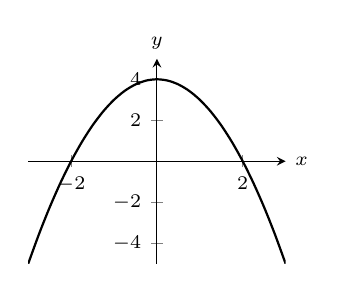
\begin{tikzpicture}
\begin{axis}[width=.4\textwidth,tick label style={font=\scriptsize },
	axis y line=middle,axis x line=middle,
    ymin=-5,ymax=5,
	xmin=-3,xmax=3,name=myplot]
\addplot [draw={\colorone},smooth,thick,domain=-3:3] {4-x^2};
\end{axis}
\node [right] at (myplot.right of origin) {\scriptsize $x$};
\node [above] at (myplot.above origin) {\scriptsize $y$};
\end{tikzpicture}
}{concave up on $(-2,2)$;\\
concave down on $(-\infty,-2)$; $(2,\infty)$;\\
inflection points when $x=\pm2$}

\exercise{Given the graph of $\fp$, identify the concavity of $f$ and its inflection points.\\
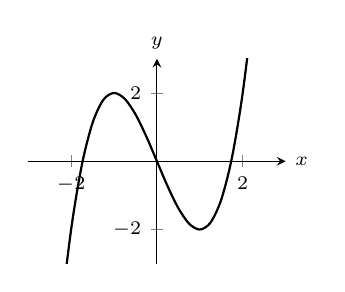
\begin{tikzpicture}
\begin{axis}[width=.4\textwidth,tick label style={font=\scriptsize },
	axis y line=middle,axis x line=middle,
    ymin=-3,ymax=3,
	xmin=-3,xmax=3,name=myplot]
\addplot [draw={\colorone},smooth,thick,domain=-3:3] {x*(x^2-3)};
\end{axis}
\node [right] at (myplot.right of origin) {\scriptsize $x$};
\node [above] at (myplot.above origin) {\scriptsize $y$};
\end{tikzpicture}
}{concave up on $(-\infty,-1)$; $(1,\infty)$;\\
concave down on $(-1,1)$;\\
inflection points when $x=\pm1$}

% cut for parity
%\exercise{Given the graph of $f$, identify the concavity of $f$ and its inflection points.\\
%\begin{tikzpicture}
%\begin{axis}[width=.4\textwidth,tick label style={font=\scriptsize },
%	axis y line=middle,axis x line=middle,
%    ymin=-5,ymax=5,
%	xmin=-3,xmax=3,name=myplot]
%\addplot [draw={\colorone},smooth,thick,domain=-3:3] {x^2*(x^2-6)+4};
%\end{axis}
%\node [right] at (myplot.right of origin) {\scriptsize $x$};
%\node [above] at (myplot.above origin) {\scriptsize $y$};
%\end{tikzpicture}
%}{concave up on $(-\infty,-1)$; $(1,\infty)$;\\
%concave down on $(-1,1)$;\\
%inflection points when $x=\pm1$}

\input{exercises/03-04-exset-01}

\input{exercises/03-04-exset-02}

%\printreview

%\exercise{Consider $f(x) = x^2-3x+5$ on $[-1,2]$; find $c$ guaranteed by the Mean Value Theorem.}{$c=1/2$}

%\exercise{Consider $f(x) = \sin x$ on $[-\pi/2,\pi/2]$; find $c$ guaranteed by the Mean Value Theorem.}{$c=\pm \cos^{-1}(2/\pi)$}
